\documentclass[ngerman,hyperref={pdfpagelabels=false}]{beamer}

% -----------------------------------------------------------------------------

\graphicspath{{images/}}

% -----------------------------------------------------------------------------

\usetheme{KIT}

\setbeamercovered{transparent}
%\setbeamertemplate{enumerate items}[ball]

\newenvironment<>{KITtestblock}[2][]
{\begin{KITcolblock}<#1>{#2}{KITblack15}{KITblack50}}
{\end{KITcolblock}}

\usepackage[ngerman,english]{babel}
\usepackage[utf8]{inputenc}
\usepackage[TS1,T1]{fontenc}
\usepackage{array}
\usepackage{multicol}
\usepackage[absolute,overlay]{textpos}
\usepackage{beamerKITdefs}
\usepackage{amsfonts}

\newcommand{\code}[1]{\texttt{#1}}


\pdfpageattr {/Group << /S /Transparency /I true /CS /DeviceRGB>>}	%required to prevent color shifting withd transparent images


\title{Tutorium 17, \#9, Weihnachtstutorium}
\subtitle{Max Göckel-- \textit{uzkns@student.kit.edu}}

\author[Max Göckel]{Max Göckel}
\institute{Institut für Theoretische Informatik - Grundbegriffe der Informatik}

\TitleImage[width=\titleimagewd,height=\titleimageht]{titel}

\KITinstitute{Institut f\"ur Theoretische Informatik}
\KITfaculty{Fakult\"at f\"ur Informatik}

% -----------------------------------------------------------------------------

\begin{document}
\setlength\textheight{7cm} %required for correct vertical alignment, if [t] is not used as documentclass parameter


% title frame
\begin{frame}
  \maketitle
\end{frame}


%Algorithmen
\begin{frame}
  \frametitle{Algorithmen}
Ein Algorithmus ist eine Vorschrift um ein Problem zu lösen, dabei überführt ein Algorithmus eine Eingabe in eine Ausgabe.\\
Diese Vorschrift besteht dabei aus endlich vielen elementaren Einzelschritten, die dann zusammen den Algorithmus formen.\\
\ \\
Man kann sich einen Algorithmus wie ein Kochrezept vorstellen das die Zutaten (Eingabe) in ein Endprodukt (Ausgabe) überführt.
\end{frame}


%Hoare Kalkühl
\begin{frame}
  \frametitle{Hoare-Kalkül: Grundlagen}
Um die Korrektheit eines Algorithmus zu beweisen haben wir das \emph{Hoare-Kalkül}.\\
Dies beweist die Korrektheit eine Algorithmus indem es Aussagen (sog. "Zusicherungen") über den Zustand der Ausführung macht.\\
\ \\
Eine Aussage zeigt dabei die Korrektheit eines Algorithmus bis zu dem jeweiligen Punkt.\\
\end{frame}


%Hoare Tripel
\begin{frame}
  \frametitle{Hoare-Kalkül: Tripel}

Ein Hoare-Tripel besteht aus zwei Zusicherungen und einem Stück Programmcode:\\
\ \\
\begin{itemize}
	\item \{P\}: Vorbedingung
	\begin{itemize}
		\item P soll wahr sein bevor der Programmcode beginnt
	\end{itemize}
	\item S: Codesegment
	\begin{itemize}
		\item Ein Stück Algorithmus - eine oder mehrere Zeilen vom Code
	\end{itemize}
	\item \{Q\}: Nachbedingung
	\begin{itemize}
		\item Ist P wahr und wurde S ausgeführt so soll nun Q wahr sein.
	\end{itemize}
\end{itemize}
\ \\
Eine Hoare-Zusicherung hat also die Form $\{P\} S \{Q\}$
\end{frame}


%Hoare Regeln
\begin{frame}
  \frametitle{Hoare-Kalkül: Tripel}

Für die Tripel gelten bestimmte Regeln ($ {HT}_1, {HT}_2, {HT}_3 $):\\
\ \\
\begin{itemize}
	\item[$HT_1$] Gilt $P' \rightarrow P \wedge Q \rightarrow Q'$ und ist $\{P\} S \{Q\}$ korrekt, so ist auch $\{P'\} S \{Q'\}$ korrekt
	\item[$HT_2$] $\{P\} S_1 \{Q\}$ und $\{Q\} S_2 \{R\}$ sind korrekt $\rightarrow$ $\{P\}S_1 S_2 \{R\}$ ist korrekt
	\item[$HT_3$] Bei der Zuweisung $x \leftarrow \beta$ kann man aus der Nachbed. eine Vorbed. erstellen indem man $x$ mit $\beta$ substituiert
\end{itemize}
\end{frame}


%Hoare H_1
\begin{frame}
  \frametitle{Hoare-Kalkül: $HT_1$}
Wir probieren immer eine möglich ungenaue Vorbedingung und eine möglichst genaue Nachbedingung finden.\\
Wieso?\\
\ \\
 \begin{itemize}
	\item[Vorbedingung] Unser Algorithmus soll für möglichst viele Eingaben das richtige Ergebnis produzieren \\ $\Rightarrow$ Möglichst allgemeine Vorbedingung finden
	\item[Nachbedingung] Über das Ergebnis der Überführung soll man so viele Aussagen wie möglich treffen können \\ $\Rightarrow$ Möglichst genaue Nachbedingung finden
\end{itemize}
\end{frame}


%Beispiel
\begin{frame}
  \frametitle{Hoare-Kalkül: Beispiel}
$S_1 = b \leftarrow a$, \\
$S_2 = c \leftarrow b$, \\
$Q = \{ c = 5 \}$.\\
\ \\

$\{ ?_1 \} $\\
$S_1$\\
$\{ ?_2 \} $\\
$S_2$\\
$Q $\\
\ \\
Finde $?_1, ?_2$ heraus.
\end{frame}


%LÖSUNG
\begin{frame}
  \frametitle{Hoare-Kalkül: Beispiel}
$S_1 = b \leftarrow a$, \\
$S_2 = c \leftarrow b$, \\
$Q = \{ c = 5 \}$.\\
\ \\

$\{ ?_1 \} $\\
$b \leftarrow a; $\\
$\{ ?_2 \} $\\
$c \leftarrow b; $\\
$Q $\\
\ \\
Finde $?_1, ?_2$ heraus.\\
$?_1: \{ a = 5 \}$\\
$?_2: \{ b = 5 \}$
\end{frame}


%Aufgabe
\begin{frame}
  \frametitle{Hoare-Kalkül: Aufgabe}
$S = x \leftarrow (x - y) \cdot (x+y)$, \\
$Q = \{ x+ y^{2} \neq 0 \}$. \\
\ \\
Bestimme die Vorbedingung $P$.
\end{frame}


%LÖSUNG
\begin{frame}
  \frametitle{Hoare-Kalkül: Aufgabe}
$S = x \leftarrow (x - y) \cdot (x+y)$, \\
$Q = \{ x+ y^{2} \neq 0 \}$. \\
\ \\
Einsetzen ($HT_3$) in $Q$:\\
$\{ (x-y) \cdot (x+y) + y^2 \neq 0 \} \Leftrightarrow $ \\
$\{  x^2 - y^2 + y^2 \neq 0 \} \Leftrightarrow $ \\
$\{  x^2 \neq 0 \} = P$
\end{frame}


%If Then Else
\begin{frame}
  \frametitle{Hoare-Kalkül: Verzweigungen}
In Algorithmen gibt es auch Verzweigungen der Form \\
\code{if B then S else T}. Diese können mit Hoare-Tripeln ausgewertet werden.\\
\ \\
$\{ P \}$ Verzweigung $\{ Q \}$ wahr $ \Leftrightarrow \{ P \wedge B \} S \{ Q \}$ u. $\{ P \wedge \neg B \} T \{ Q \}$ wahr\\
d.h. für eine Verzweigung sind beide Fälle wahr wenn man die Bedigung im \code{if}-Teil umdreht.\\
\end{frame}


%while-Loops
\begin{frame}
  \frametitle{Hoare-Kalkül: Schleifen}
Neben Verzweigungen gibt es auch Schleifen. Wir reden hier nur von Schleifen der Form \code{while B do S}, wo das Tripel $\{ I \wedge B \} S \{ I \}$ gelten soll. Dabei ist $I$ die Schleifeninvariante. Eine Schleifeninvariante ist eine Bedigung, die vor und nch jedem Durchlauf der Schleife gültig ist.\\
\ \\
Gilt die Invariante $I$ so gilt auch $\{I\}$ Loop $\{ I \wedge \neg B \}$
\end{frame}


%Beispiele
\begin{frame}
  \frametitle{Hoare-Kalkül: Schreibweise}
\begin{columns}
\column[T]{.50\textwidth}
\textbf{if-then-else}\smallskip \\
$\{ P \}$ \\
if $B$ then \\
\hspace*{5mm} $\{ P \wedge B \}$ \\
\hspace*{5mm} $ S $ \\
\hspace*{5mm} $\{ Q \}$ \\
else \\
\hspace*{5mm} $\{ P \wedge \neg B \}$ \\
\hspace*{5mm} $ T $ \\
\hspace*{5mm} $\{ Q \}$ \\
$\{ Q \}$


\column[T]{.50\textwidth}
\textbf{while-do}\smallskip \\
$\{ I \}$ \\
while $B$ do \\
\hspace*{5mm} $\{ I \wedge B \}$ \\
\hspace*{5mm} $ S $ \\
\hspace*{5mm} $\{ I \}$ \\
$\{ I \wedge \neg B \}$ \\
\end{columns}
\end{frame}


%Beispiele

\begin{frame}
  \frametitle{Hoare-Kalkül: Beispiele}
\begin{columns}
\column[T]{.50\textwidth}
\textbf{if-then-else}\smallskip \\
if $(x > y)$ then \\
\hspace*{5mm} $z \leftarrow y$ \\
else \\
\hspace*{5mm} $z \leftarrow x$ \\
Mit Eingabe $a,b$ für $x,y$. \\

\column[T]{.50\textwidth}
\textbf{while-do}\smallskip \\
$s \leftarrow a$ \\
$y \leftarrow b$ \\
for $(i \leftarrow 0$ to $b-1)$ do \\
\hspace*{5mm} $s \leftarrow s+1$ \\
\hspace*{5mm} $y \leftarrow y-1$ \\
\end{columns}
\end{frame}


%Graphen
\begin{frame}
  \frametitle{Graphen: Grundlagen}
Ein Graph ist eine Struktur, die eine Menge von Elementen und eine Verbindung dieser Elemente darstellt.\\
Dabei ist $V$ die Menge aller Elemente auf dem Graph (die Knoten, engl. Vertices) und E die Verbindung zwischen den Elementen (die Kanten, engl. Edges)\\
\ \\
Formal:\\
Ein Graph G ist ein Tupel $(V, E)$ mit $V$ Menge der Knoten und $E$ Menge der Verbindungen/Kanten.
\end{frame}


%Gerichtet, ungerichtet
\begin{frame}
  \frametitle{Graphen: Gerichtet vs. Ungerichtet}
\begin{columns}
\column[T]{.50\textwidth}
\textbf{Gerichtet}\smallskip \\
\begin{itemize}
	\item $G = (V, E)$
	\item $E \subseteq V \times V$
	\item E ist also Teilmenge des karth. Produktes und besteht aus Tupeln der Form $(A, B)$
	\item $(A, B)$ heißt damit "von A nach B"
	\item Die Relation wird durch einen Pfeil $ A \rightarrow B$ ausgedrückt
\end{itemize}

\column[T]{.50\textwidth}
\textbf{Ungerichtet}\smallskip \\

\begin{itemize}
	\item $G = (V, E)$
	\item $E \subseteq \{ \{x, y\} | x,y \in V \}$
	\item E Teilmenge einer Menge aus Mengen der Form $\{A, B\}$
	\item $\{A, B\}$ heißt damit "A und B sind verbunden"
	\item Die Relation wird durch einen Strich $ A - B$ ausgedrückt
\end{itemize}

\end{columns}
\end{frame}


\begin{frame}
\frametitle{Beispielgraph}

\begin{figure}[htbp] 
  \centering
     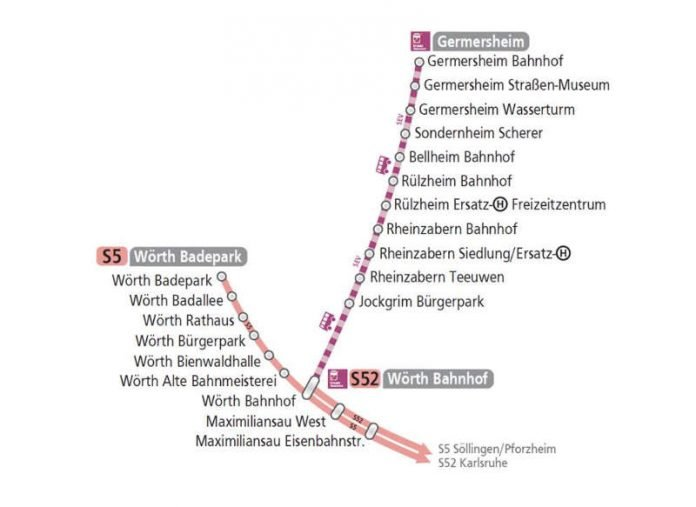
\includegraphics[width=0.7\textwidth]{images/kvv.jpg}
  \caption{Ausweichfahrplan S5/S52 März 2017}
  \label{fig:Bild1}
\end{figure}
\end{frame}


%Teilgraphen
\begin{frame}
  \frametitle{Graphen: Teilgraphen}
Ein Teilgraph ist ähnlich einer Teilmenge nur ein bestimmter Abschnitt vom Graph. Dabei ist egal ob der Teilgraph zusammenhängt (Alle Knoten verbunden sind) oder nicht.\\
\ \\
Formal: \\
Ist $G = (V, E)$ ein gerichteter Graph so ist $T = (V', E')$ mit $V' \subseteq V$ und $E' \subseteq E \cap (V' \times V')$ ein Teilgraph von G. \\
Ist G ungerichtet so ist $E' \subseteq E \cap \{ \{ x,y \} | x,y \in V' \}$ \\
\end{frame}


%Pfade und Wege
\begin{frame}
  \frametitle{Graphen: Wege und Pfade}
Sind zwei Knoten mit einer Kante verbunden, so sind sie \emph{adjazent}.\\
\ \\
In einem gerichteten Graph ist ein Pfad von A nach B eine Liste aus zueinander adjazenten Knoten. Die Länge des Pfades ist dabei die Anzahl der Kanten zwischen den Knoten.\\
\ \\
In einem ungerichteten Graph ist ein Weg von A nach B ein ungerichteter Pfad von A nach B.\\
\ \\

\begin{itemize}
	\item Gerichteter Graph $G = (V, E)$ \emph{streng zusammenhängend} $\Leftrightarrow \forall A,B \in V \exists$ Pfad $A \rightarrow B$
	\item Ungerichteter Graph $G = (V, E)$ \emph{zusammenhängend} $\Leftrightarrow$ $G$ ist aus einem Stück
\end{itemize}
\end{frame}


%Grade
\begin{frame}
  \frametitle{Graphen: Grade}

Der Grad eines Knoten in einem gerichteten Graph ist die Anzahl der Pfeile die von ihm weggehen und zu ihm führen.\\
\begin{itemize}
	\item Der Eingangsgrad $d^{-}(D)$ ist die Anzahl der Kanten die in D hineingehen
	\item Der Ausgangsgrad $d^{+}(D)$ ist die Anzahl an Kanten die aus D weggehen
	\item der Grad $d(D)$ ist $d^{+}(D) + d^{-}(D)$, also alle Kanten kombiniert
\end{itemize}
\ \\
Für ungerichtete Graphen gibt es keinen Eingangs-/Ausgangsgrad, also ist der Grad $d(D)$ die Anzahl der Kanten in denen D vorkommt.

\end{frame}

\begin{frame}
\frametitle{Adjazenzmatrizen}
Man kann eine Graph nicht nur als Zeichnung darstellen, sondern auch als Matrix.\\
Diese Matrizen heißen Adjazenzmatrizen, sie sind immer quadratisch und gehören eindeutig zu einem Graphen.\\
\ \\
An einer Adjazenzmatrix kann man die Kanten eines Graphen ablesen.
\end{frame}


%Aufbau Matrix
\begin{frame}
\frametitle{Adjazenzmatrizen: Aufbau}
\begin{itemize}
\item Jede Zeile i steht für einen Knoten $k_i \in V$
\item Jede Spalte j steht für die von $k_i$ direkt erreichbaren Knoten
\begin{itemize}
	\item $ 1 \Leftrightarrow \exists \{ k_i , k_k \} \in E $, es existiert eine Kante zwischen den beiden Knoten
	\item $ 0 \Leftrightarrow \neg \exists \{ k_i , k_k \} \in E $, es existiert keine Kante
\end{itemize}
\end{itemize}
\end{frame}


%Beispiel
\begin{frame}
\frametitle{Adjazenzmatrizen: Beispiel}

Die folgende Beispielmatrix beschreibt einen Graphen mit 4 Knoten:\\
\ \\

$A = 
\begin{pmatrix}
1 & 1 & 1 & 0 \\
0 & 0 & 1 & 1 \\
0 & 1 & 1 & 0 \\
0 & 0 & 0 & 0
\end{pmatrix}
$ 
\end{frame}


%%Beispiel
\begin{frame}
\frametitle{Adjazenzmatrizen: Ungerichtete Graphen}
Bei ungerichteten Graphen ändert sich die Adjazenzmatrix nicht, die einzige Besonderheit ist dass sie symmetrisch ist.\\
\ \\
Die folgende Beispielmatrix beschreibt den selben Graphen wie eben als ungerichteten Graph: \\
\ \\

$B = 
\begin{pmatrix}
1 & 1 & 1 & 0 \\
1 & 0 & 1 & 1 \\
1 & 1 & 1 & 0 \\
0 & 1 & 0 & 0
\end{pmatrix}
$ 
\end{frame}


%Aufgabe
\begin{frame}
\frametitle{Adjazenzmatrizen: Aufgaben}
Bestimme den Graph anhand der Adjazenzmatrix:\\
$ X =
\begin{pmatrix}
1 & 1 & 1 & 0 & 0 \\
1 & 0 & 1 & 1 & 0 \\
1 & 1 & 0 & 1 & 1 \\
0 & 1 & 1 & 1 & 0 \\
0 & 0 & 1 & 1 & 0
\end{pmatrix}
$ 
\end{frame}

%LÖSUNG
\begin{frame}
\frametitle{Adjazenzmatrizen: Lösung}
$ A_C =
\begin{pmatrix}
1 & 1 & 1 & 0 & 0 \\
1 & 0 & 1 & 1 & 0 \\
1 & 1 & 0 & 1 & 1 \\
0 & 1 & 1 & 0 & 1 \\
0 & 0 & 1 & 1 & 0
\end{pmatrix}
$ \\
\ \\
$ A_D =
\begin{pmatrix}
0 & 0 & 1 & 0 & 0 & 0 \\
0 & 0 & 0 & 1 & 0 & 0 \\
0 & 0 & 0 & 0 & 1 & 0 \\
0 & 0 & 0 & 0 & 0 & 1 \\
1 & 0 & 0 & 0 & 0 & 0 \\
0 & 1 & 0 & 0 & 0 & 0 
\end{pmatrix}
$
\end{frame}


\end{document}
